\section{Date: 2026-10-20}
\noindent \textbf{Series ID: COLATZ11} 

\noindent This series is titled Import Price Index by Origin (NAICS): Agriculture, Forestry, Fishing and Hunting for Latin America and has a frequency of Monthly. The units are Index Jun 2012=100 and the seasonal adjustment is Not Seasonally Adjusted.The observation start date is 2012-06-01 and the observation end date is 2026-09-01.The popularity of this series is 1. \\ 

\noindent \textbf{Series ID: WFRBLN40059} 

\noindent This series is titled Checkable Deposits and Currency Held by the 50th to 90th Wealth Percentiles (DISCONTINUED) and has a frequency of Quarterly. The units are Millions of Dollars and the seasonal adjustment is Not Seasonally Adjusted.The observation start date is 1989-07-01 and the observation end date is 2022-04-01.The popularity of this series is 2. \\ 

\subsection{Raw Regression}
\noindent Regresses the two series against each other directly. A significant result here can come just as easily from both series sharing a long-run trend as from any real relationship.

\begin{center}
\begin{tabular}{lclc}
\toprule
\textbf{Dep. Variable:}        & value\_fred\_WFRBLN40059 & \textbf{  R-squared:         } &     0.267   \\
\textbf{Model:}                &           OLS            & \textbf{  Adj. R-squared:    } &     0.248   \\
\textbf{Method:}               &      Least Squares       & \textbf{  F-statistic:       } &     13.87   \\
\textbf{Date:}                 &     Tue, 20 Oct 2026     & \textbf{  Prob (F-statistic):} &  0.000635   \\
\textbf{Time:}                 &         15:55:02         & \textbf{  Log-Likelihood:    } &   -553.28   \\
\textbf{No. Observations:}     &              40          & \textbf{  AIC:               } &     1111.   \\
\textbf{Df Residuals:}         &              38          & \textbf{  BIC:               } &     1114.   \\
\textbf{Df Model:}             &               1          & \textbf{                     } &             \\
\textbf{Covariance Type:}      &        nonrobust         & \textbf{                     } &             \\
\bottomrule
\end{tabular}
\begin{tabular}{lcccccc}
                               & \textbf{coef} & \textbf{std err} & \textbf{t} & \textbf{P$> |$t$|$} & \textbf{[0.025} & \textbf{0.975]}  \\
\midrule
\textbf{const}                 &   -1.261e+06  &     4.72e+05     &    -2.672  &         0.011        &    -2.22e+06    &    -3.06e+05     \\
\textbf{value\_fred\_COLATZ11} &     1.62e+04  &     4349.040     &     3.724  &         0.001        &     7390.953    &      2.5e+04     \\
\bottomrule
\end{tabular}
\begin{tabular}{lclc}
\textbf{Omnibus:}       &  8.566 & \textbf{  Durbin-Watson:     } &    0.269  \\
\textbf{Prob(Omnibus):} &  0.014 & \textbf{  Jarque-Bera (JB):  } &    7.873  \\
\textbf{Skew:}          &  1.067 & \textbf{  Prob(JB):          } &   0.0195  \\
\textbf{Kurtosis:}      &  3.413 & \textbf{  Cond. No.          } & 1.28e+03  \\
\bottomrule
\end{tabular}
%\caption{OLS Regression Results}
\end{center}

Notes: \newline
 [1] Standard Errors assume that the covariance matrix of the errors is correctly specified. \newline
 [2] The condition number is large, 1.28e+03. This might indicate that there are \newline
 strong multicollinearity or other numerical problems.

\begin{figure}
\centering
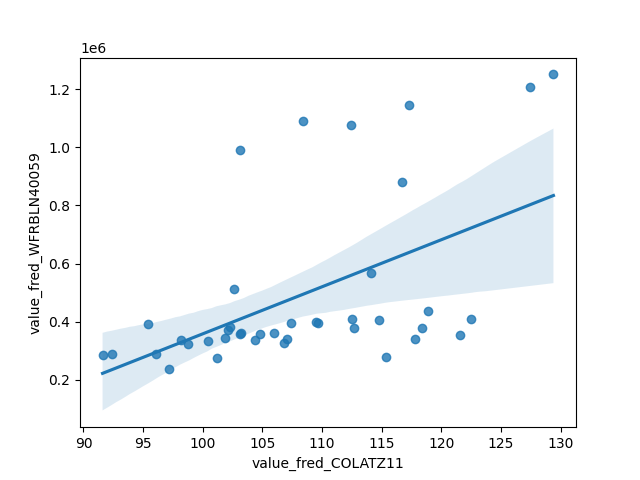
\includegraphics[scale = 0.9]{plots/plot_2026-10-20.png}
\caption{Raw Regression Plot for 2026-10-20}
\end{figure}
\newpage
\subsection{Detrended Regression}
\noindent Regresses the residuals of each series after removing its own linear time trend, so a shared trend can no longer drive the result on its own. A relationship that stays significant here is better evidence of a genuine link between the two series.

\begin{center}
\begin{tabular}{lclc}
\toprule
\textbf{Dep. Variable:}                   & value\_fred\_WFRBLN40059\_detrended & \textbf{  R-squared:         } &     0.001   \\
\textbf{Model:}                           &                 OLS                 & \textbf{  Adj. R-squared:    } &    -0.025   \\
\textbf{Method:}                          &            Least Squares            & \textbf{  F-statistic:       } &   0.03202   \\
\textbf{Date:}                            &           Tue, 20 Oct 2026          & \textbf{  Prob (F-statistic):} &    0.859    \\
\textbf{Time:}                            &               15:55:02              & \textbf{  Log-Likelihood:    } &   -543.18   \\
\textbf{No. Observations:}                &                    40               & \textbf{  AIC:               } &     1090.   \\
\textbf{Df Residuals:}                    &                    38               & \textbf{  BIC:               } &     1094.   \\
\textbf{Df Model:}                        &                     1               & \textbf{                     } &             \\
\textbf{Covariance Type:}                 &              nonrobust              & \textbf{                     } &             \\
\bottomrule
\end{tabular}
\begin{tabular}{lcccccc}
                                          & \textbf{coef} & \textbf{std err} & \textbf{t} & \textbf{P$> |$t$|$} & \textbf{[0.025} & \textbf{0.975]}  \\
\midrule
\textbf{const}                            &   -5.959e-08  &      3.1e+04     & -1.92e-12  &         1.000        &    -6.28e+04    &     6.28e+04     \\
\textbf{value\_fred\_COLATZ11\_detrended} &    -859.3401  &     4802.520     &    -0.179  &         0.859        &    -1.06e+04    &     8862.854     \\
\bottomrule
\end{tabular}
\begin{tabular}{lclc}
\textbf{Omnibus:}       &  0.421 & \textbf{  Durbin-Watson:     } &    0.106  \\
\textbf{Prob(Omnibus):} &  0.810 & \textbf{  Jarque-Bera (JB):  } &    0.579  \\
\textbf{Skew:}          &  0.150 & \textbf{  Prob(JB):          } &    0.749  \\
\textbf{Kurtosis:}      &  2.493 & \textbf{  Cond. No.          } &     6.46  \\
\bottomrule
\end{tabular}
%\caption{OLS Regression Results}
\end{center}

Notes: \newline
 [1] Standard Errors assume that the covariance matrix of the errors is correctly specified.

\begin{figure}
\centering
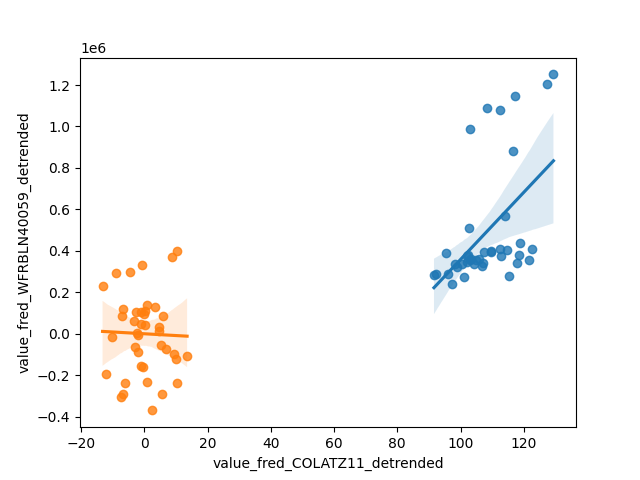
\includegraphics[scale = 0.9]{plots/plot_2026-10-20_detrended.png}
\caption{Detrended Regression Plot for 2026-10-20}
\end{figure}
\newpage
